\section{提案されている手法}
本稿で実装する,Using QUIC to traverse NATsで提案されているP2P通信の確立手法は以下の二つである.なお,手法2については本稿での実装は完了しなかった.

\subsection{手法1: ICEプロトコルを用いた通信確立}
\begin{figure}[h]
  \centering
  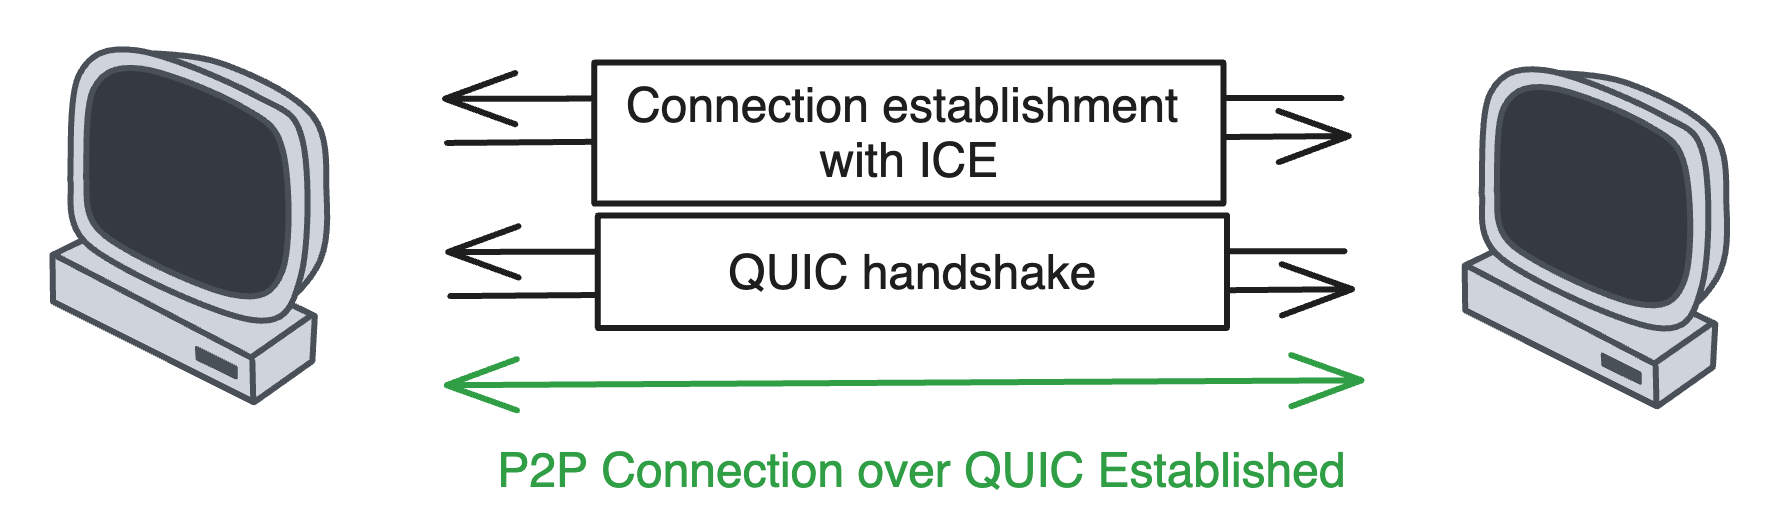
\includegraphics[width=\linewidth]{figs/approach-1.png}
  \caption{ICEプロトコルを用いたQUIC上でのP2P通信確立}
  \label{fig:one}
\end{figure}
図~\ref{fig:one}に示すように,先行事例で示したICEプロトコルを用いてUDP上でP2P通信を確立し,その通信の上でQUICハンドシェイクを開始する.QUICはUDPの上に成り立つプロトコルであるためこの手法は成立する.

この手法は既存のICEプロトコル実装を利用でき,またQUIC自体の変更は必要ないためプロトコルを拡張できない環境でのユースケースが想定される.

\subsection{手法2: QUICのみを用いた通信確立}
\begin{figure}[h]
  \centering
  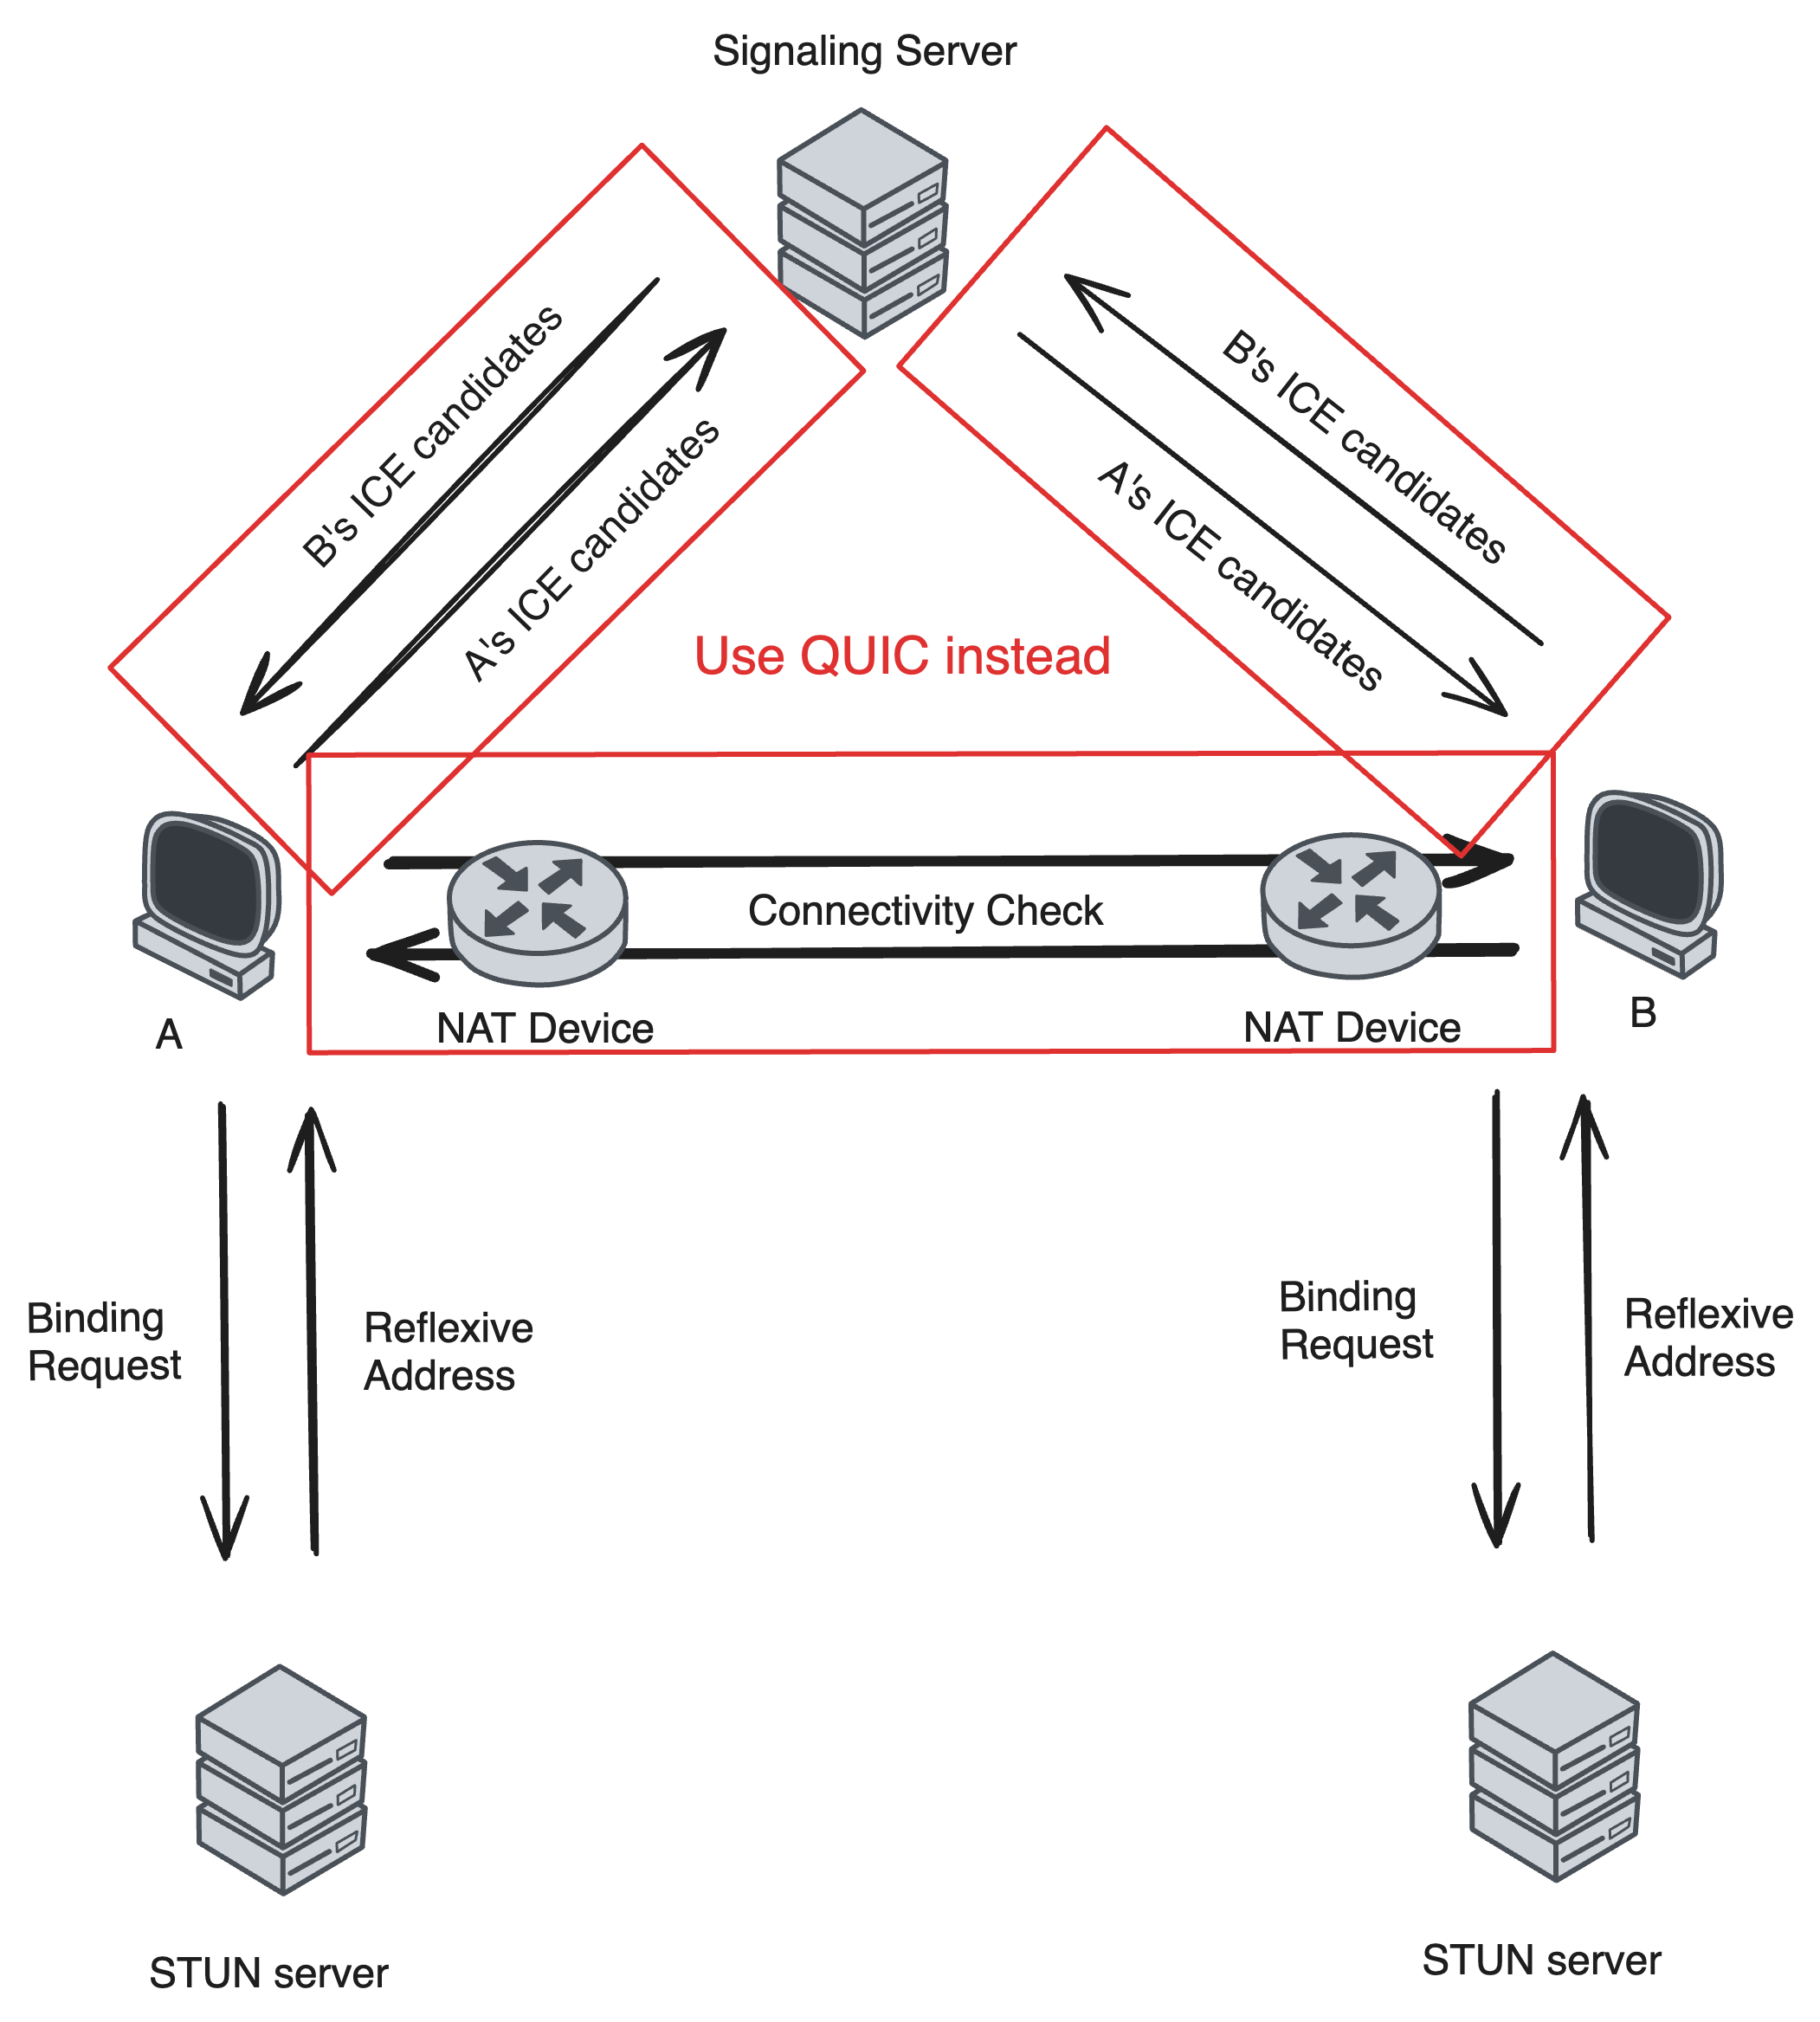
\includegraphics[width=\linewidth]{figs/approach-2.png}
  \caption{QUICのみを用いたP2P通信確立}
  \label{fig:two}
\end{figure}
図~\ref{fig:two}に示すように,この手法ではICEプロトコルが司るアドレス交換や接続性チェックを全てQUICの上で行う.アドレスペアの優先順位を決定するアルゴリズムや通信確立の手順はICEプロトコルを踏襲するため,ICE over QUICの実装とも言える.接続性チェックに関しては,QUICのハンドシェイクに含まれるPath Validationフレームを用いる.これにより,接続性チェックとハンドシェイクを併せて行うことができ,手法1に比べて通信確立がより効率的になる.

一方で,既存のICEプロトコルの実装は使えないため,実装の際はICEプロトコルをQUIC上で再実装する必要がある.またQUICの拡張が必要なため,プロトコルの拡張ができない環境ではこの手法を利用することはできない.
